% !TEX root = ../thesis.tex
After we looked at the general feasibility of the cumulant LBM scheme, we now have a look at a standard benchmark in fluid dynamics, Schaefer-Turek,~\cite{schafer1996benchmark}.
There, they collected computations for various flows around cylinders and rectangles in $2$ and $3$ spatial dimensions under varying conditions and on different grids.

\begin{figure}
  \centering
  % !TEX root = ../../thesis.tex


\begin{tikzpicture}

\draw[color=gray, style=dashed] (-0.5,2) -- (2,2);
\draw[color=gray, style=dashed] (-0.5,2.5) -- (2,2.5);
\draw[color=gray, style=dashed] (2,-0.5) -- (2,2);

\fill[pattern=north east lines, pattern color=gray] (0,0) rectangle (10,-0.2);
\fill[pattern=north east lines, pattern color=gray] (0,4.1) rectangle (10,4.3);
\draw (0,0) .. controls (1,1.55) and (1,2.55) .. (0,4.1);
\draw (0,0) -- (10,0);
\draw (0,4.1) -- (10,4.1);
\draw (0,0) -- (0,4.1);

\draw[->] (0,4.1/2) -- (0.75,4.1/2);
\draw[->] (0,2.73) -- (0.66,2.73);
\draw[->] (0,1.36) -- (0.66,1.36);
\draw[->] (0,3.4) -- (0.4,3.4);
\draw[->] (0,0.68) -- (0.4,0.68);

\node (u) at (0.3,2.3) {$\vec{u}$};


\draw[->] (-0.5,-0.7) -- (-0.5,5);
\draw[->] (-0.5,-0.7) -- (10.5,-0.7);

\node (y) at (-0.5,5.2) {$y$};
\node (x) at (10.7,-0.7) {$x$};


\node (nullx) at (0,-0.95) {$0$};
\draw[-] (-0.55,0) -- (-0.45,0);

\node[anchor=east] (nully) at (-0.5,0) {$0$};
\draw[-] (0,-0.65) -- (0,-0.75);

\fill[pattern=north east lines, pattern color=gray, draw=black]  (2,2) circle (0.5);

\node at (2,-0.95) {$0.2$};
\draw[-] (2,-0.65) -- (2,-0.75);
\node  at (10,-0.95) {$2.2$};
\draw[-] (10,-0.65) -- (10,-0.75);

\node[anchor=east]  at (-0.5,2) {$0.2$};
\draw[-] (-0.55,2) -- (-0.45,2);

\node[anchor=east]  at (-0.5,2.5) {$0.25$};
\draw[-] (-0.55,2.5) -- (-0.45,2.5);

\node[anchor=east]  at (-0.5,4.1) {$0.41$};
\draw[-] (-0.55,4.1) -- (-0.45,4.1);
\fill[ draw=black]  (2,2) circle (0.02);

\end{tikzpicture}

  \caption{Setup for the Schaefer-Turek benchmark}
\label{fig: schaeferTurek}
\end{figure}

Figure~\ref{fig: schaeferTurek} gives an overview of the problem we examine.
We have a channel flow at a low Reynolds number of $100$, similar to the Poiseuille flow.
This time however, there is a cylinder placed slightly off center and exposed to the parabolic inflow.
The quantity of interest is the lift it experiences\footnote{Forces are calculated via a momentum exchange, which is independent of the collision we use and not elaborated further.}.

Again, a grid study was done, this time controlling the radius of the sphere and scaling the computational domain accordingly.
This brings one caveat however:
As we scale our spatial coordinates, we also have to scale our timesteps, according to equation~\eqref{eq: relation between stepsizes}.
Hence, for double the resolution in each of the spatial dimensions, we don't need $4$ times but $8$ times the computation time.
Thus, any savings in spatial resolution will pay off greatly in the final computation times.


\begin{figure}
  \centering
  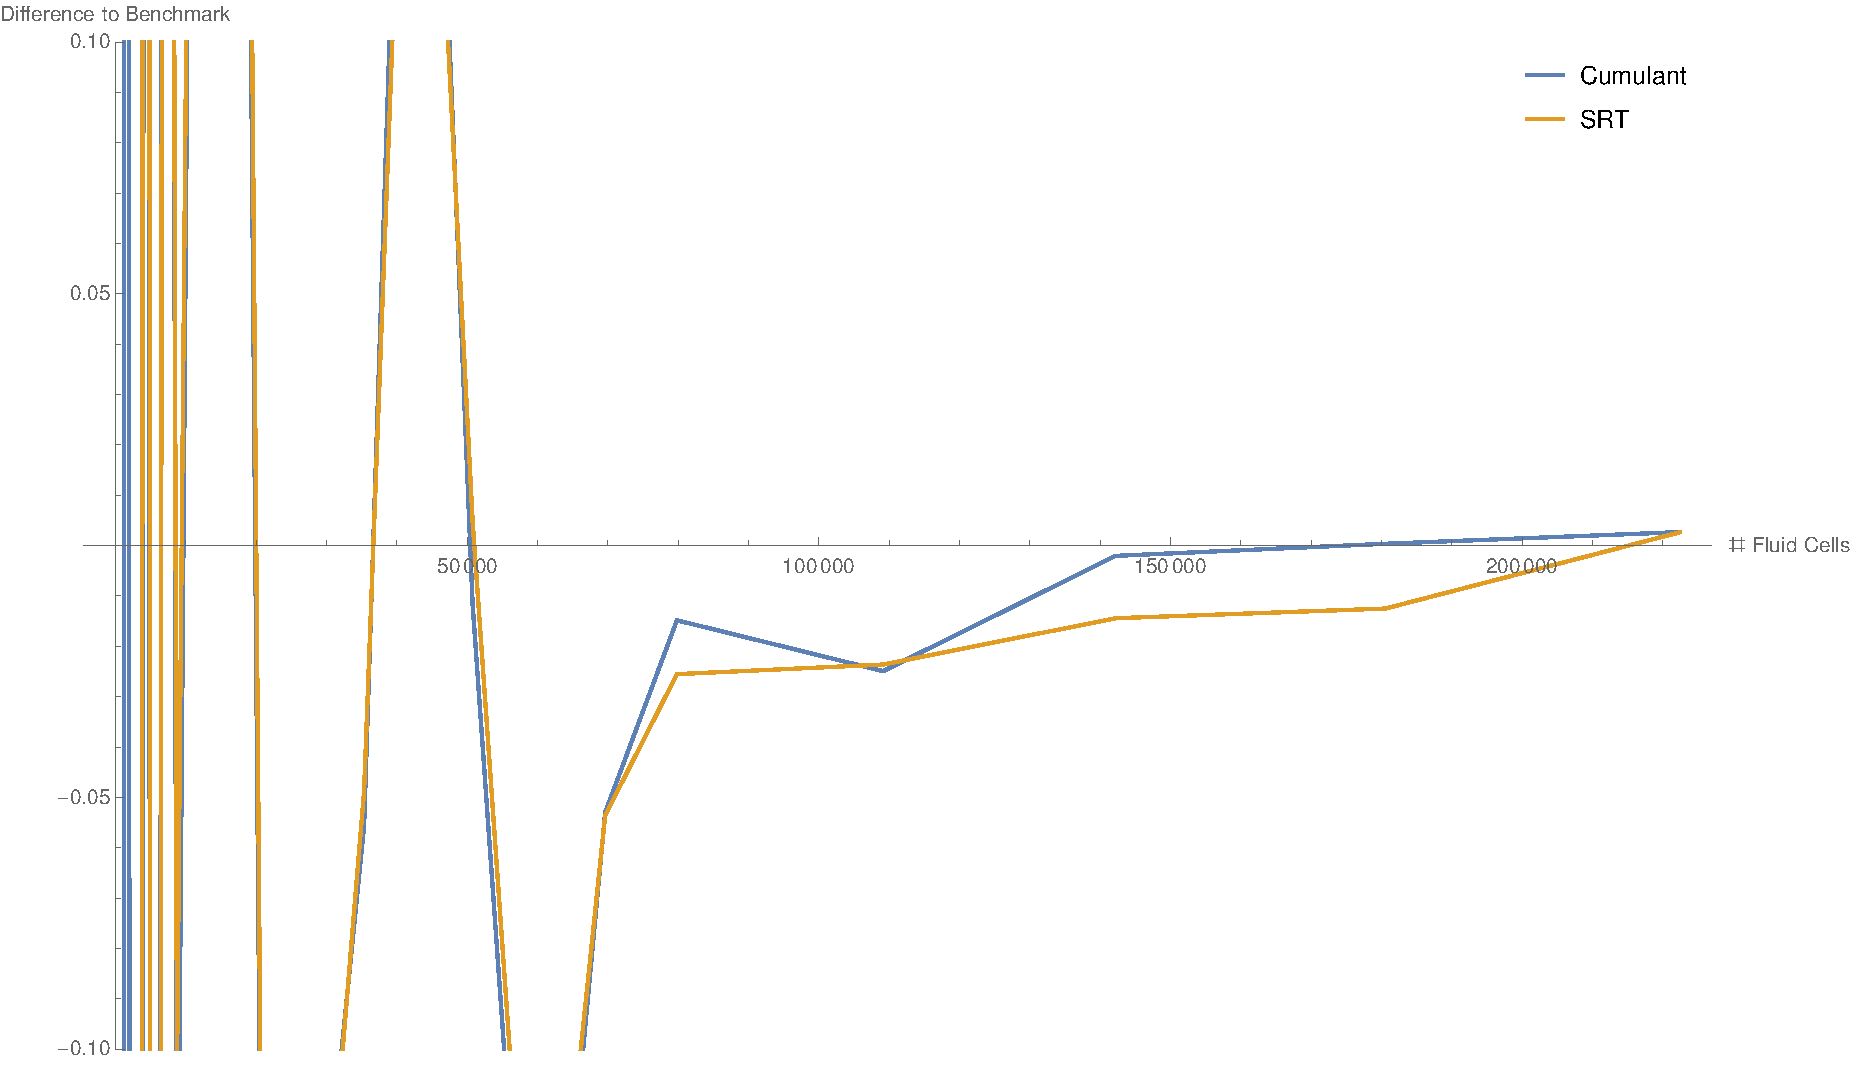
\includegraphics[width=\linewidth]{../figures/schaeferTurekLift_nrFluidVsDiff.pdf} % chktex 11
  \caption{Difference between the lift force of a sphere in relation to the computational domain.}
\label{fig: schaefer turek nrFluidVsDiff}
\end{figure}

Going over to the actual computation results, we find the situation depicted in Figure~\ref{fig: schaefer turek nrFluidVsDiff}.
The x-Axis is chosen to depict the number of fluid cells instead of the radius of the sphere to allow the comparison to the study in~\cite{schafer1996benchmark}, where they also plotted against the degrees of freedom.
The y-Axis is centered around $0.0110$, the value they got for their biggest resolution.
At the lower end of the scales, the lift is quite unsteady, presumably caused by the still bad approximation of the cylinder.
Afterwards, SRT stays a bit longer at the line marked by the benchmark, whereas the cumulants go faster in the direction of the wanted result.

\begin{figure}
\centering
\begin{subfigure}{.48\textwidth}
  \centering
  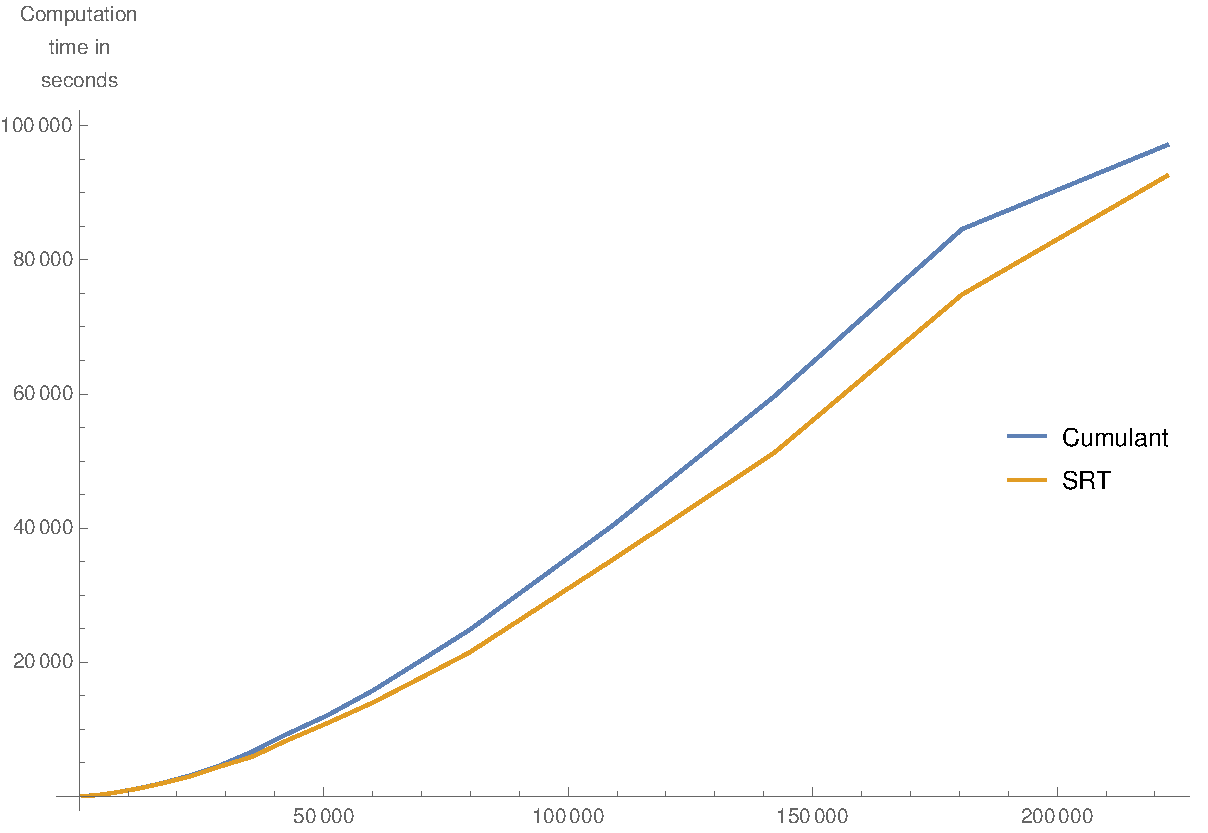
\includegraphics[width=\linewidth]{../figures/schaeferTurekLift_domainVsTime.pdf} % chktex 11
  \caption{Relation between the size of the computational domain and the computation time for cumulants and SRT.}
\label{fig: schaefer turek domain vs time}
\end{subfigure}\hfill
\begin{subfigure}{.48\textwidth}
  \centering
  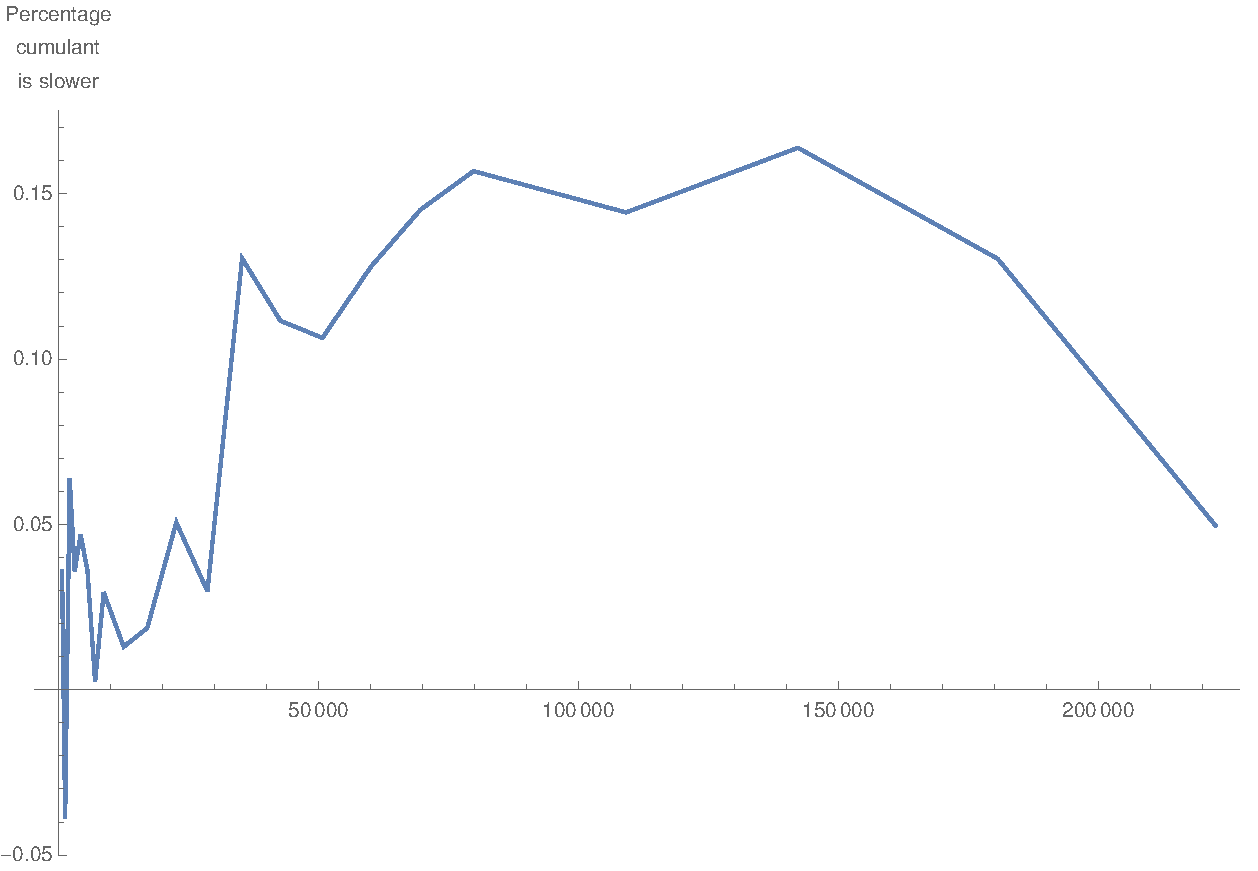
\includegraphics[width=\linewidth]{../figures/schaeferTurekLift_performanceGap.pdf} % chktex 11
  \caption{Percentage of raw additional time needed for cumulant collision versus SRT.}
\label{fig: schaefer turek time percentage}
\end{subfigure}
\caption{Analysis of the difference in computation time. X-Axis is both times the number of fluid cells.}
\label{fig: time analysis cumulant vs SRT}
\end{figure}

This is all well, but we don't know yet if we sacrifice a whole lot of performance and thus just compare apples with oranges.
Figure~\ref{fig: time analysis cumulant vs SRT} wants to shed a bit of light onto this topic.
The cumulant method is indeed a bit slower, around $10-15\%$, which is not all that bad.

However, we have to treat this not just with a bit of caution, but a whole lot.
The implementation of both methods was done conscientious to not introduce major pitfalls and slowdowns.
It cannot be ruled out though, that one method allows for more low level optimizations than the other, tilting the result.
However, a recent experimental implementation of the cumulants in the highly optimized \href{http://walberla.net/index.html}{waLBerla}\footnote{widely applicable Lattice Boltzmann from Erlangen} comparing it to the native SRT showed a drop in MLUPs\footnote{Mega-lattice-updates per second} of about $50\%$ which is honestly quite amazing for an unoptimized comparison.

\begin{figure}
  \centering
  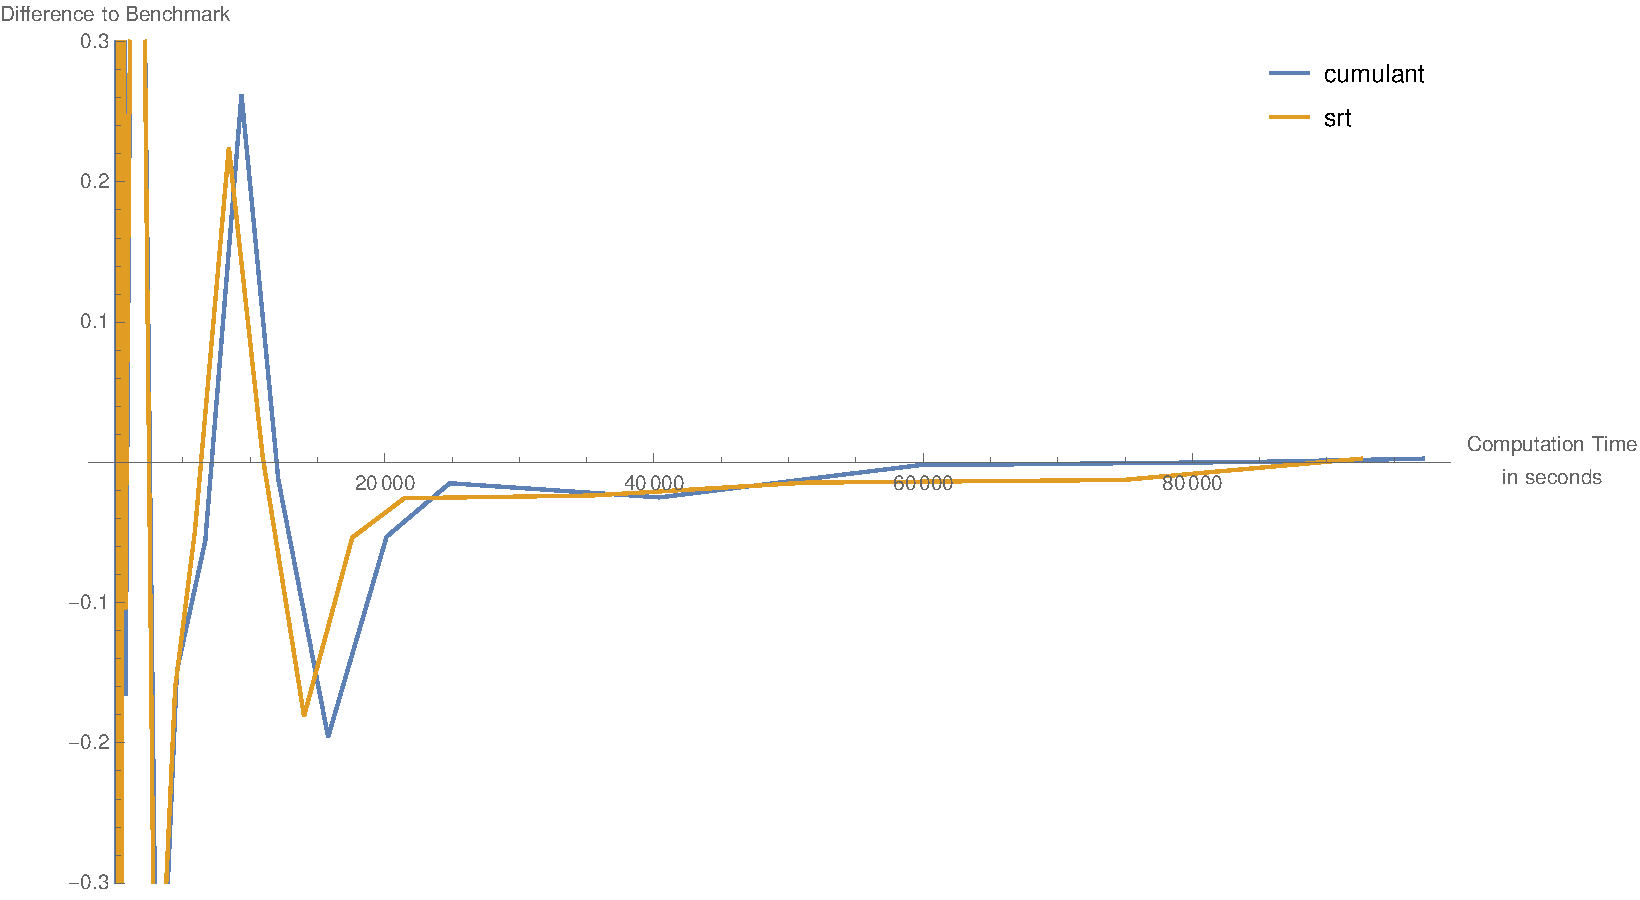
\includegraphics[width=\linewidth]{../figures/schaeferTurekLift_timeDifference.pdf} % chktex 11
  \caption{Difference between the lift force of a sphere in relation to the computational time.}
\label{fig: schaefer turek time difference}
\end{figure}

So, indeed it is feasible to compare the methods normalized with their runtimes, which was done in Figure~\ref{fig: schaefer turek time difference}.
Also here, the cumulant method features an earlier convergence to the final result.
\par

We can conclude, that the cumulant LBM is feasible if not superior to SRT even at low Reynolds numbers.
What's left is the analysis if cumulants also hold their promise if we crank it up.
